\subsection{平均场近似}
前一章演示了如何从简单和复杂流体的粒子模型构建统计场理论. 如何在平衡状态下分析这些场理论, 并提取有关聚合物流体结构和热力学性质的有用信息, 是目前研究讨论的热点. \\

第四章的场论模型将相关的配分函数一般表示为一个或多个化学势场$w(\br)$上的函数积分, 即\\
\begin{equation}
	\mathcal{Z}=\int  \ \exp(-H[w])\ \mathcal{D}w \label{配分函数}
\end{equation}
其中$H[w]$是一个有效的哈密顿量, 它是场变量的非局部泛函, 通常是复的(不是严格实的). $H[w]$的形式依赖于特定的相互作用和用于构建场理论的链模型, 因此对聚合物的结构、分子量、多分散性、组成等都很敏感. 为了计算某些可观测$G$的集合平均, 我们应用公式\\
\begin{equation}
	\langle G[w]\rangle = \mathcal{Z}^{-1}\int  G[w]\ \exp(-H[w])\ \mathcal{D}w \label{可观测G}
\end{equation}
通过与$\mathcal{Z}$的热力学联系公式计算自由能和导数量, 需要计算方程(\ref{配分函数})给出的泛函积分. 同样地, 利用相应的密度算子$G[w]$计算方程(\ref{可观测G}), 将流体结构计算为两个泛函积分的比值. \\

实际上, 对于非平凡的三维流体模型, 这些函数积分都不能用封闭的形式来计算. 但是, 有几种选择:\\

1.\ \ 生成精确场理论的数值逼近. \\

2.\ \ 采用解析近似来简化场理论, 然后用解析方法计算感兴趣的量. \\

3.\ \ 采用解析近似来简化理论, 然后用数值方法从简化理论中提取信息. \\
\\
第一种策略, 我们称之为“场理论模拟”(FTS)技术, 是第六章的主题. 本章讨论了第二和第三种方法. \\
\subsubsection{平均场近似:一般想法}
最重要的解析近似技术是平均场近似, 这在聚合物物理学文献中也被称为自洽场理论(Edwards, 1965;de Gennes, 1969). 这一技术在许多物理环境中得到了广泛的应用, 也许最显著的是在相变理论中(AMIT, 1984;Parisi, 1988;Goldenfeld, 1992). 在这种情况下, 平均场近似等于假设单场构型$w^*(\br)$控制方程(\ref{配分函数})和(\ref{可观测G})中的泛函积分. 这种场构型是通过要求$H[w]$相对$w(\br)$的变化是平稳的得到的, 即\\
\begin{gather}
	\left. \frac{\delta H[w]}{\delta w(\br)}\right|_{w=w^*} =0 \label{H[w]相对w(r)的变化}
\end{gather}
在得到这个方程的“平均场”势$w^*(\br)$后, 可以完成近似通过\\
\begin{gather}
	\mathcal{Z} \approx \exp(-H[w^*]),\quad \langle G[w]\rangle \approx G[w^*]
\end{gather}
如果$\mathcal{Z}$代表正则配分函数, 则Helmholtz自由能由$\beta A = -ln\mathcal{Z} = H[w^*]$立即得到. \\

在平均场近似下, 除特殊构型$w^*(\br)$外, 势场的所有构型都被忽略. 对于原子或小分子流体, 这种忽略所有“场波动(filed fluctuations)”的近似通常是相当差的. 这是因为在液体密度下, 原子或小分子的典型配位数(typical coordination number)很低, $\sim 10$, 所以当粒子的位置发生变化时, 粒子的电位会发生很大的波动. 事实上, 这些强的局域场波动是产生描述液体原子尺度结构的密度关联(dendity correlations)的原因(Hansen和McDonald, 1986). \\

由于配位数仍然很小, 在聚合物溶液或原子尺度的熔体中, 平均场近似也是不准确的. 然而, 在\textbf{介观尺度}上, 由于聚合物线圈相互渗透的能力, 情况发生了质的变化. 从介观角度看, 聚合物流体中有效配位数的一个有用定义是\\
\begin{gather}
	C=\rho_c R_g^3
\end{gather}
其中$\rho_c=n/V$是链的平均数密度, $R_g$表示聚合物的旋转半径. 因此, $C$对应于一条兴趣链所占体积中(估计为$R_g^3$)的(其他)聚合物链的平均数. 这一有效的配位数可以是非常大的浓缩溶液或聚合物熔体的高分子质量. 例如, 在均聚物熔体中, $\rho_c=1/(v_0N)$, 其中$v_0$是每个统计段所占的体积, N是每条链的段数. 由于聚合物在$R_g=b(N/6)^{1/2}$的熔体中是渐近理想的, 因此$C\sim (b^3/v_0)N^{1/2}$. 因此, 在熔体条件下, 有效配位数随着分子量的平方根的增大而增大. 因此, 在介观尺度下, 每种聚合物的波动都随着分子量的增加而减小, 因为势场的变化是通过接触越来越多的周围链来平均的. 这构成了一个标准论点, 即平均场近似对于高分子量聚合物的浓缩溶液或熔体是准确的(de Gennes, 1979年). \\


平均场近似的实现需要求解方程(\ref{H[w]相对w(r)的变化})来获得“平均场”$w^*(\br)$. 对于实际的模型, 这类方程是非线性的, 非局部的, 并且不服从封闭形式的解析解.然而, 对于包含精确场理论的复杂泛函积分, 平均场方程仍然是一个很大的简化. 在讨论求解平均场方程的数值和近似解析策略之前, 先讨论与复平面场理论的解析结构有关的一些一般性问题, 以及方程(\ref{H[w]相对w(r)的变化})多解的存在性和意义. \\
\subsubsection{场理论的解析结构}
如果有效的哈密顿量$H[w]$是严格实的, 则方程(\ref{H[w]相对w(r)的变化})的物理解将对应于$H$的局部最小值, 从而对应于自由能的平均场近似的最小值, 即$\beta A \approx H $. 然而, 由于$H[w]$的复杂性使第四章所描述的模型也变得复杂. 方程(\ref{H[w]相对w(r)的变化})物理上有意义的解可以脱离实轴, 这样$w^*$可以是纯虚的, 也可以是复的. 配分函数$\mathcal{Z}$是实的, 因此$H[w^*]$也必须是实的. 同样, 对于任何真实的物理可观测的$G$, $G[w^*]$都必须是实的. \\

利用$w^*$附近$H[w]$的解析结构的优点, 将复平面上方程(\ref{H[w]相对w(r)的变化})的近似解统称为鞍点. 由于这个原因, 平均场近似也被称为鞍点近似. 正如之前所述, 聚合物中的平均场近似的另一个等价名称是自洽场理论. 这个名称来源于这样的概念, 即聚合物段在位置$\br$处所受到的平均势场$w^*(\br)$是由(\ref{H[w]相对w(r)的变化})“自洽”决定的. \\

为了实现平均场近似并清楚什么时候平均场近似有效, 检验定义在模型中的有效哈密顿量的解析结构是非常重要的. 我们用一个简单的一维“玩具”模型来说明\\
\begin{equation}
\mathcal{Z} = \int_{-\infty}^{\infty}\ \exp[-H(w)]\ dw \label{玩具模型}
\end{equation}
其有效哈密顿量为\\
 \begin{equation}
 H(w) = p \ \left[iw+ \frac{1}{2} w^2\right] \label{有效哈密顿量}
 \end{equation}
这里$p>0$是一个实常数. 积分路径是实$w$轴, 但是因为哈密顿量中$i=\sqrt{-1}$, $H(w)$是复的. 然而, 配分函数是实的, 因为它由$\mathcal{Z}=(2\pi/p)^{1/2} \exp(-p/2)$决定. \\

方程(\ref{玩具模型})的被积函数, $\exp[-H(w)]$是变量$w$在复平面上的一个解析函数. 本文从复积分的柯西定理出发, 定义$\mathcal{Z}$时积分路径由沿着实轴可变形为复$w$平面上的任意曲线, $w = w_R +iw_I$,当$w_R \rightarrow  \pm \infty$时与实轴相连, 正如图\ref{复平面w}中标有$\Gamma_1$的曲线, 图中第二条曲线$\Gamma_2$在$w_R=\pm X$处通过垂直段连接到实心轴上, 故应用柯西定理给出了另一种表达式\\
\begin{equation}
\mathcal{Z} = \int_{\Gamma_1} \exp [-H(w)] \ dw = \lim_{X \rightarrow +\infty} \int_{\Gamma_2} \exp[-H(w)] \ dw   \label{Z的另一种表达式}
\end{equation}

只有当沿$\Gamma_1$或$\Gamma_2$的积分比沿实轴的积分更容易时, $\mathcal{Z}$的上述表达才会有用. 根据因子$\exp(-ipw)$, 原始积分沿积分路径$w=w_R$有一个\textbf{振荡积分}. 虽然对于眼前的简单模型来说, 这并不是问题, 但在大多数实际情况下, 振荡积分可能导致相当大的数值困难. 人们可能会问, 是否有可能找到一条曲线$\Gamma$, 使得$H(w)$的虚部, 即所谓的相$H_I(w_R,w_I)$, 沿着积分路径是常数. 如果可以找到的话, 这种数值困难的可能性就会被消除. 实际上, 这一过程是对方程(\ref{Z的另一种表达式})这类积分渐近分析的最速下降(或鞍点)法的基础. \\

最速下降法中, 至少有一个大的$p$, $p\gg1$, 沿恒定相轮廓$\Gamma$的积分是由哈密顿量的实部$H_R$局部最小值决定的. 如果$H(w)$是解析的, 那么由柯西-黎曼方程得到这些局部最小值$w^*$对应于复导数消失的鞍点:\\
\begin{equation}
\left. \frac{dH(w)}{dw}\right|_{w=w^*} = 0 \label{复导数为0}
\end{equation}
部分相关知识说明:\\
 \begin{equation}
 \begin{aligned}
 H(w) &= ipw+\frac{pw^2}{2}\\
 &=ip(w_R+iw_I)+\frac{pw_R^2}{2}-\frac{pw_I^2}{2}-ipw_Rw_I\\
 &=\frac{pw_R^2}{2}-\frac{pw_I^2}{2}-pw_I +ipw_R(1-w_I)\\
 \end{aligned}
 \end{equation}
 故$H_R = \frac{pw_R^2}{2}-\frac{pw_I^2}{2}-pw_I$,  $H_I=pw_R(1-w_I)$,\\

 \begin{gather}
\frac{ \partial{H_R} }{\partial{W_R}}=pw_R\\
\frac{ \partial{H_R} }{\partial{W_I}}=0\\
\frac{ \partial{H_I} }{\partial{W_R}}=ip(1-w_I)\\
\frac{ \partial{H_I} }{\partial{W_I}}=0
\end{gather}
又由柯西黎曼方程得$w_R = 0$,$w_I=0$,故得方程(\ref{复导数为0})


在方程(\ref{有效哈密顿量})的情况下, 玩具模型被视为在虚轴$w^* = -i$处具有单个鞍点. 也可以看出, 计算二阶鞍点时, 二阶导数$H''(w^*)$不为0, 两个恒定相位曲线相交. 其中一条曲线的两个部分由鞍点描述, 对应于$H_R$远离鞍点增加的上升曲线. 类似地, 另一曲线的两个部分是下降曲线, 沿着该曲线$H_R$减小. 对于玩具模型, $H_I(w_R,w_I) = p \ w_R(1+w_I)$, 使得在鞍点处$H_I = 0$. 有$w^* = -i$发出的两条恒定相曲线对应于$w_R=0$和$w_I=-1$. 它很容易验证$w_R=0$的两个部分都是下降曲线, $w_I=-1$产生两个上升曲线. 这些在图\ref{复平面w}中示出. 应该注意的是, 上升曲线与$\Gamma_2$的分段一致, 平行于实轴. \\

\begin{figure}[H]
      \centering
      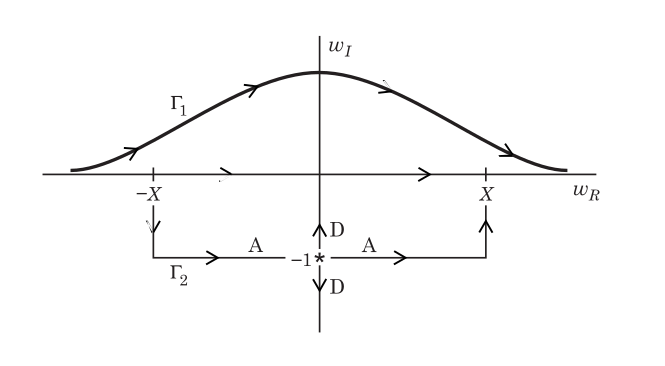
\includegraphics[width=12cm]{./figures/1.png}
      \caption{复$w$平面, $w =w_R + iw_I$, 表明由(\ref{玩具模型})和(\ref{有效哈密顿量})定义的玩具模型的积分路径. 最初的积分路径是沿着实轴, $w_I=0$. 柯西定理允许积分变形成任意轮廓$\Gamma_1$, 它在$w_R \rightarrow \pm \infty $处与实轴相连. 同样, 当$X \rightarrow +\infty$时, 分段轮廓$\Gamma_2$也可应用. 玩具模型在虚轴$w^*= -i$处有一个鞍点, 由星号标记. 通过鞍点的恒定相曲线具有$H_I=0$, 对应于线$w_I=-1$和$w_R=0$. 上升曲线标记$A$和下降曲线标记$D$}
      \label{复平面w}
\end{figure}
上升曲线是我们主要感兴趣的曲线, 因为它们可以通过轮廓$\Gamma_2$连接到原始的积分路径, 并对配分函数产生一个有限的结果. 当$ X \rightarrow +\infty$时在$w_R=\pm X$ 处轮廓片段的分布衰减为$\sim \exp(-pX^2/2)$,所以可以忽略. 这样, 我们就可以通过$w =x -i$, 将原来的积分正式地转化为恒定相路径$\Gamma$上的积分\\
\begin{equation}
\begin{aligned}
\mathcal{Z} &= \int_\Gamma \exp[-H(w)] \ dw = \int_\infty^\infty \exp[-H_R(x,-1)] \ dx\\
& =\int_\infty^\infty \exp[-p(1+x^2)/2] \ dx \label{恒定相路径积分}
\end{aligned}
\end{equation}
由于相因子$\exp(iH_I)$沿着积分路径不变, 所以最终积分不再具有振荡积分. 该积分可以用方程(B.1)得到精确结果$\mathcal{Z}=(2\pi/p)^{1/2}\exp(-p/2)$. 一个重要的观测结果是, 对于较大的$p$, 沿着恒定相路径上的积分由鞍点$x=0$时$H_R$的局部极小值決定. $p\rightarrow +\infty$時, 拉普拉斯型积分不能解析计算, 为其提供了渐近展开. \\

本文讨论的一维“玩具”模型有几个要点, 可以立即推广到像方程(\ref{配分函数})一样的高维的静态场理论中:\\

$\bullet$ 在定义的配分函数时, 场$w(\br)$的每个自由度的初始积分路径是沿实轴的. 尽管如此, 对于一个解析积分$\exp(-H[w])$, 它是有用的, 至少对多维复平面上的通过一个或多个鞍点$w^*(\br)$的恒定相“上升”轮廓(面)的积分路径有用. 相因子$\exp(iH_I[w])$沿这样的轮廓是恒定的, 从而消除了被积函数的振荡. \\

 $\bullet$通过对第四章模型的检验, 容易证明统计权重$\exp(-H[w])$和$\exp(-H_G[w])$是$w$的解析泛函. 因此, 上述变形对于所有模型都是可能的. 但是, 应该指出的是, 只有在巨正则系综中哈密顿量才解析, 且在正则系宗中, $H[w]$具有奇点,限制了解析区域. \\

$\bullet$鞍点场构型$w^*$对泛函积分在恒定相轮廓上变形有重要贡献, $w^*$代表平均场解. 在恒定相(上升)流形上, $H_R[w]$在鞍点上具有局部最小值. 鞍点场构型对积分的影响程度取决于一个“金兹伯格参数”的值, 类似于玩具模型中的$p$. 实际上, 很容易证明配位数$C=\rho_cR_g^3$是第四章中描述的许多模型的相关参数. 因此, $C\rightarrow +\infty$时, 这些模型的平均场近似变得精确. \\

$\bullet$在进行计算之前, 先确定复平面上鞍点的定性位置和方向是很有用的. 例如, 在模型$A$中, 要求$H[w^*]$或$H_G[w^*]$是实的意味着几乎所有鞍点$w^*(\br)$必须是纯虚的. 对于模型$B-E$, $w_{-}^*$和$w_{+}^{*}$分别是纯实的和纯虚的.利用虚轴上的松弛方案计算一个纯虚的鞍点是很方便的, 这是一个与物理积分路径正交的搜索方向. 对于这样的方案, 重要的是要认识到这很可能是$H_R[w]$的下降方向, 所以我们应该寻找一个局部最大值, 而不是一个局部最小值!\\
\subsubsection{多解}
对于大多数感兴趣的流体模型, 方程(\ref{H[w]相对w(r)的变化})有多个解, 对应于多个鞍点. 一个广义分类方案将这类鞍点识别为各向同性的, 即$w^*(\br)$独立于位置$\br$, 或各向异性的—$w(\br)$具有明显的位置相关性. 各向同性鞍点往往可以解析确定, 而各向异性鞍点通常需要数值方法进行计算. \\

一般来说, 人们可以将一个纯态鞍点与流体的每一个稳定或亚稳定相关联. 例如, $AB$型两嵌段聚合物的模型具有“纯态”鞍点, 可与无序相($D$), 层状相($L$), 柱状相($C$), 螺旋二十四面体($G$)和球形($S$)中间相关联. $L$, $C$, $G$和$S$鞍点是各向异性的且准周期的;稳定的S鞍点具有体心三次(bcc)对称. 对模型$E$其他纯态鞍点是已知的, 例如双金刚石($DD$)和超细粉体($HPL$)对称性的点已经被计算出来. 平均场理论中, 这些在整个$\mathcal{X}N$和$f$的参数空间都是亚稳态的. \\

各向异性的纯态点不一定是周期性的. 在这种情况下, 各向异性的结构通常是由适用于模型的边界条件决定的. 例如, 模型A在描述一个好溶剂中均聚合物的解时, 当在狄利克雷边界条件的约束几何中求解时, 它有一个唯一的、非均匀的纯态点$w^*(z)$. $\tilde{\rho}(z;[iw^*])$给出了平均场近似中与此势对应的段密度分布, 其中$\tilde{\rho}$是方程(4.75)的密度算子. 这类不均匀剖面的数值例子见图\ref{剖面}. 
\begin{figure}[H]
       \centering
        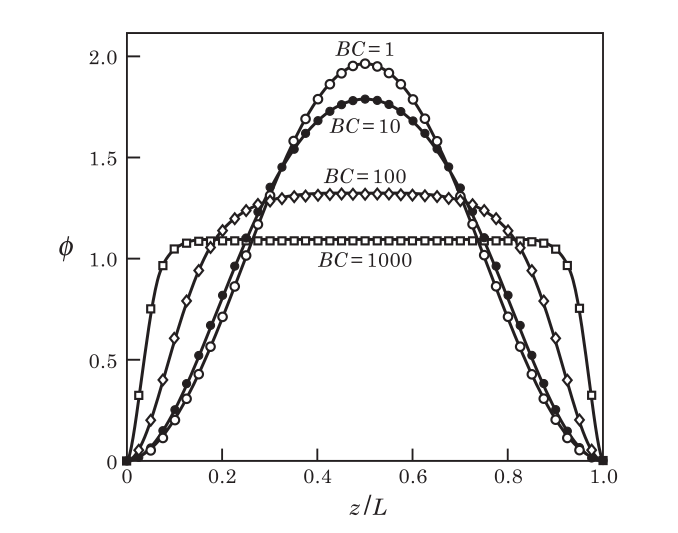
\includegraphics[width=12cm]{./figures/2.png}
       \caption{在一个简单的几何中求解模型$A$得到的平均场约密度剖面. 对于$BC=1$(开圆), $BC=10$(填充圆), $BC=100$(开菱形)和$BC=1000$(开方形)的数值结果. 固体线表示符合基于基态优势近似的解析表达式. 转载自Alexander-Katz等人. (2003年)}
        \label{剖面}
 \end{figure}

纯态鞍点是唯一的, 除了平移和旋转不改变能量$H[w^*]$. 即使在一类空间周期结构中, 对于一个特定的复杂流体模型, 也很难计算和评估所有纯态鞍点的稳定性. 在实际应用中, 我们主要感兴趣的是模型参数空间中具有一定稳定性区域对应的鞍点. 幸运的是, 最稳定的鞍点(即$H[w^*]$值最低的点)通常也是能量图形中吸引力最大的点, 因此可以通过大型单元模拟来识别它们, 使$w$场从随机初始构型中放松下来(参见章节5.3.4). 更普遍地, 对任意流体模型求方程(\ref{H[w]相对w(r)的变化})最小能量纯态解是全局优化中的一个不能解决的问题(Nocedal 和 Wright, 1999). \\

除了“纯态”点外, 还可以找到对应于缺陷态的方程(\ref{H[w]相对w(r)的变化})的各向异性的解. 它们之所以如此命名, 是因为它们反映了另一种完美的周期结构中的拓扑缺陷. 例如, 类似于二维六状晶体的位错, 两嵌段共聚物的柱状薄膜可能具有所谓的位错(Hammond等人, 2003年). 当圆柱体与薄膜的平面垂直排列时, 这样的面内位错会反映出相邻的柱状共聚物的“旋错对”, 一个是5个近邻, 另一个是7个. 如圖\ref{方格图}中所示, 除了这些旋错对外, 所有其他柱状都有6个最近的近邻. 由于纯态鞍点具有较低的能量, 与缺陷态对应的鞍点(如刚刚描述的位错)通常是亚稳的. 然而, 对于带有边界条件的方程(\ref{H[w]相对w(r)的变化})纯态解是不适应的, 如球体表面的晶化情况(Nelson, 1983), “缺陷状态”鞍点可以变得稳定. 也有理论和实验支持玻璃形成的系统拥有大量的(在系统尺寸下)的再结晶缺陷态(Monasson,1995年;Zhang和Wang, 2005). 冷却后, 这样的系统会被困在其中一种不稳定的状态中, 从而产生一种玻璃化转变. \\
\begin{figure}[H]
        \centering
         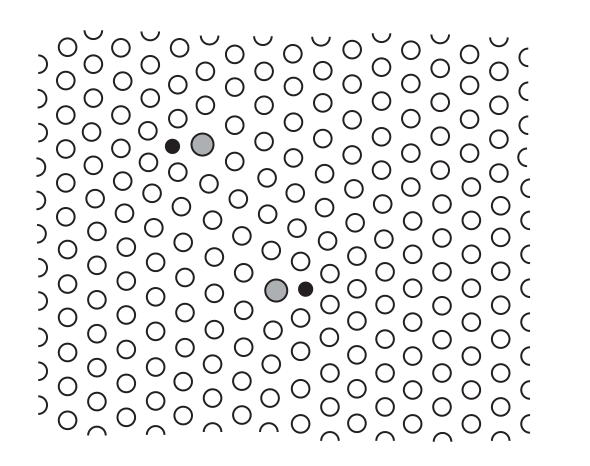
\includegraphics[width=12cm]{./figures/3.png}
    \caption{包含两个位错的柱状形成的块状聚合物的二维六状方格图. 每个位错本身就是一个由5个近邻(黑色)和7个近邻(灰色)的柱状构成的旋错对. 所有柱状都有6个近邻(白色). 与缺陷相关的应变能导致位错与位错之间的块状再分布. 实验和数值$SCFT$计算都知道这一点, 即在7倍旋错时产生一个$\sim 20\%$的大圆柱体, 在5倍旋错时产生一个$\sim 20\%$的小圆柱体(Hammond等人, 2003年). } 
           \label{方格图}
\end{figure}


第三种类型的鞍点是两个或多个纯态共存时产生的混合状态. 例如, 一个二元共混物的模型$C$和$D$表现出两种液相共存, 在足够大的片段相互作用参数$\mathcal{X}_{AB}$下, 两种相中都很富有. 因此, 方程(\ref{H[w]相对w(r)的变化})对这些模型的正则系宗版本具有混合状态解, 反映了两个均相的共存, 组成不同, 并由一个界面分开. 对于稳定的“混合态”鞍点解, 在种类保护和应用边界条件的约束下, 通过最小面积的考虑, 可以得到界面的几何构型. 类似于纯态解, 混合状态点可以与例如均匀平移或旋转的状态点相关联. 在分离纯态相的界面没有在理想拓扑排列中配置的情况下, 也可以找到亚稳的、缺陷的、混合态的鞍点解. 

\subsubsection{均匀鞍点}
通常可以通过分析方法去定位均匀的鞍点,例如,规范模型A场理论的方程(5.3)简化为
\begin{equation}
\frac{1}{u_0}w^*(r)+i\tilde{\rho}(\br;[iw^*])=0
\end{equation}
这里,在构造泛函导数时应用了方程(4.75)中的密度算子$\tilde{\rho}(\br;[iw^*])$。在无界系统中,或在受周期性边界条件影响的立方体单元中,该方程的唯一解析解是均匀的,即$w^*(\br)=w^*$。从方程(3.25)和(3.22)得出$q(\br,s;[iw^*])=\exp(-iw^*s)$和$Q[iw^*]=\exp(-iw^*N)$以及方程(4.75)中$\tilde{\rho}(\br;[iw^*])=nN/V$,其与平均段密度$\rho_0$一致。因此,方程(5.11)简化为
\begin{equation}
w^*=-iu_0\rho_0
\end{equation}
由于排除了体积参数$u_0$和平均段密度$\rho_0$都是实数和正数的情况,因此势场的鞍点值$w^*$位于复数$w$平面的负虚轴上。这类似于第5.1.2节中讨论的玩具模型的情况。

在均匀鞍点处的规范模型A的有效哈密顿量由等式(4.72)估计为$H[w^*]=(1/2)u_0\rho_0^2V$。由此得出,聚合物溶液的Helmholtz自由能的平均场近似值由下面式子给出
\begin{equation}
A(n,V,T)=A_0+\frac{k_BT}{2}u_0\rho_0^2V
\end{equation}
这里$A_0=-k_BT\ln\calZ_0$是非相互作用聚合物的理想气体的自由能。在平均场近似中,自由能的过剩部分仅由聚合物链段之间的平均相互作用能量产生,没有考虑它们的空间相关性。

对大规范模型A重复上面的过程是很有用的。鞍点方程相当于
\begin{equation}
\frac{\delta H_G[w]}{\delta w(\br)}\bigg|_{w=w^*}=\frac{1}{u_0}w^*(\br)+i\tilde{\rho}_G(\br;[iw^*])=0
\end{equation}
其中$\tilde{\rho}_G$是方程(4.76)中给出的分段密度算子。对于均匀$w^*(\br)=w^*$,可以发现
\begin{equation}
\tilde{\rho}_G(\br;[iw^*])=zN\exp(-iw^*N)=\frac{\left\langle n\right\rangle N}{V}\equiv\rho_0
\end{equation}
其中$\left\langle n\right\rangle=zVQ[iw^*]=zV\exp(-iw^*N)$是体积$V$中聚合物的平均数,而$\rho_0$是平均链段密度。由此可见,平均场$w^*$满足以下超越方程
\begin{equation}
iw^*\exp(iw^*N)=u_0zN
\end{equation}
因为右端是实的和正的,所以该方程有唯一的解$w^*$,其位于任何聚合物活性$z$的负虚轴上。

与大规范模型A的热力学的关联通过以下公式将渗透压$\Pi$与$\calZ_G$联系起来
\begin{equation}
\begin{aligned}
\beta\Pi&=\frac{1}{V}\ln\calZ_G(z,V,T)\\
&\approx-\frac{1}{V}H_G[w^*]=\frac{\rho_0}{N}+\frac{1}{2}u_0\rho_0^2
\end{aligned}
\end{equation}
其中在上面公式的第二行中应用了平均场近似。因此,我们看到渗透压的平均场表达式是与聚合物平均密度成正比的理想气体项的总和$\rho_0/N$和与每单位体积的Helmholtz自由能中的相应项的相互作用项组成。这些当然是众所周知的结果(de Gennes,1979)。对于第四章中介绍的其他模型的均匀平均场解,可以推导出类似的表达式。

